\documentclass[__main__.tex]{subfiles}

\begin{document}
\paragraph{K-02}
Тепловое излучение и люминесценция. Равновесное тепловое излучение: свойства, спектральная плотность энергии, температура.\\

\textit{Тепловым излучением} называется испускание электро-магнитных волн телом за счет внутренней энергии. Все остальные виды излучения относятся к \textit{люминесценции}.

Тепловое излучение, находящееся в термодинамическом равновесии с веществом называют \textit{равновесным}.

\begin{statement}
Если тела находятся в термодинамическом равновесии с излучением, т.е. их температура одинакова и не меняется, то этому состоянию в пространстве между телами отвечает определенная плотность энергии теплового излучения $\operatorname{U}(T)$
\end{statement}
\begin{minipage}{.35\linewidth}
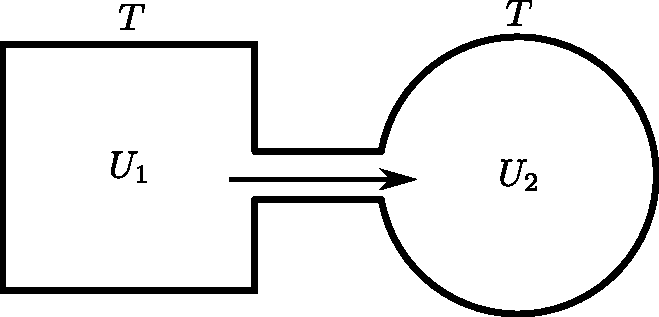
\includegraphics[width=1\linewidth]{2-reserv}
\end{minipage}
\hfill
\begin{minipage}{.6\linewidth}
\begin{proof}
Предположим обратное. Рассмотрим систему из двух связанных резервуаров, температура стенок которых одинакова, но плотность излучения различна ($U_1<U_2$). Тогда при соединении возникнет поток энергии из [1] в [2]. Следовательно, стенки [1] начинают поглощать меньше и остывают: $T_1 < T$, а в резервуаре [2] поглощение стенками возрастает, $T_2 > T$.

Получим противоречие со вторым началом термодинамики: $T_1<T_2$, следовательно температура переходит от менее нагретого тела к более нагретому.
\end{proof}
\end{minipage}\\

\textit{Объемная плотность энергии теплового излучения} -- конечная интегральная характеристика $U$, вычисляемая по формуле
\begin{gather*}
U=\int\limits_{0}^{\infty}U_\omega(T)d\omega,
\end{gather*}
где $U_\omega(T)$ -- \textit{спектральная плотность энергии ТИ}.\\

\textit{Свойства равновесного ТИ}:
\begin{enumerate}
\item
Плотность энергии равновесного ТИ и его спектральный состав не зависят от размеров и формы полости, а также от материалов полости и находящихся в ней тел.
\item
Однозначно определяется своей температурой
\item
Однородность (Равновесное ТИ имеет одинаковую объемную плотность энергии в любой точке полости)
\item
Изотропность (Спектральный состав одинаков в любой точке)
\item
Неполяризуемость (Все направления колебаний поля равновероятны)
\end{enumerate}
\end{document}